\section{Контрольная работа. Вариант \textnumero2}

\subsection{Задача \textnumero1}
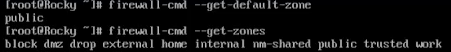
\includegraphics{1.png}
\paragraph{Решение}
Модель естесственного роста выпуска продукции при убывающей цене:
\begin{equation} \label{eq:model}
	y'(t) = mp(t)ly(t)
\end{equation}
где: \\
$m$ -- норма инвестиции, $p$ -- цена, $\frac{1}{l}$ -- норма акселерации, а $y(t)$ -- выпуск продукции, реализованный к моменту времени $t$ \\
Значит:
\begin{equation}
	y'(t) = \frac{1}{2} \cdot (2 - y(t)) \cdot 2 \cdot y(t) \\
\end{equation}

\newpage
\subsection{Задача \textnumero2}
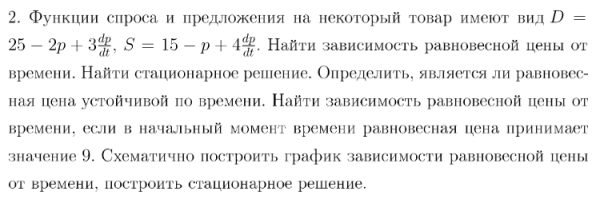
\includegraphics{2.png}

\newpage
\subsection{Задача \textnumero3}
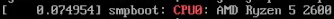
\includegraphics{3.png}
